

	\subsection{Vorticity – Wirbelstärke in der Atmosphäre}

	Die grossräumige Bewegung der Luft in der Atmosphäre lässt sich nicht nur durch Geschwindigkeit beschreiben, sondern auch durch ihre Rotationseigenschaften. Diese Eigenschaft wird durch die sogenannte \emph{Vorticity} (Wirbelstärke) quantifiziert. Physikalisch beschreibt sie die Tendenz eines Luftpakets, sich um seine eigene vertikale Achse zu drehen.

	Mathematisch ist die Vorticity definiert als Rotation des Geschwindigkeitsfeldes:
	\[
		\vec{\zeta} = \nabla \times \vec{u}.
	\]
	Für grossräumige Strömungen in der Atmosphäre betrachtet man hauptsächlich die vertikale Komponente dieser Rotation, die sogenannte \emph{relative Vorticity}. In kartesischen Koordinaten ergibt sich diese im einfachsten Fall zu:
	\[
		\zeta = \frac{\partial v}{\partial x} - \frac{\partial u}{\partial y},
	\]
	wobei \(u\) und \(v\) die zonale bzw. meridionale Windkomponente bezeichnen. Positive Vorticity (\(\zeta > 0\)) steht für eine zyklonale Rotation (auf der Nordhalbkugel gegen den Uhrzeigersinn), negative Vorticity (\(\zeta < 0\)) für eine antizyklonale Rotation (im Uhrzeigersinn).
\begin{figure}[h]
    \centering
    % Erste Reihe
    \begin{minipage}{0.32\linewidth}
        \centering
        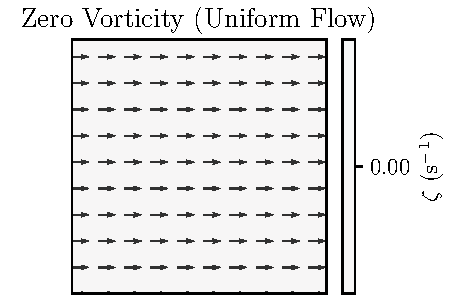
\includegraphics[width=\linewidth]{papers/rossby/images/vorticity_plot0.pdf}\\
        {\small \( \vec{u} = (2,0),\ \zeta = 0\)}
    \end{minipage}
    \begin{minipage}{0.32\linewidth}
        \centering
        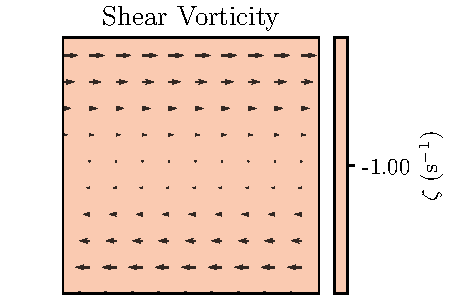
\includegraphics[width=\linewidth]{papers/rossby/images/vorticity_plot1.pdf}\\
        {\small \( \vec{u} = (y,0),\ \zeta = -1\)}
    \end{minipage}
    \begin{minipage}{0.32\linewidth}
        \centering
        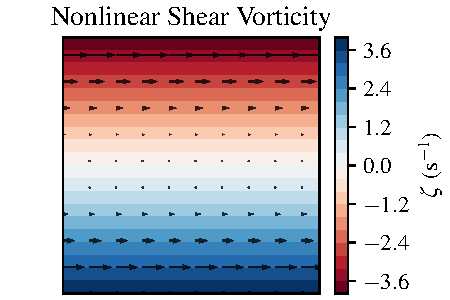
\includegraphics[width=\linewidth]{papers/rossby/images/vorticity_plot2.pdf}\\
        {\small \( \vec{u} = (y^2,0),\ \zeta = -2y\)}
    \end{minipage}

    % Zweite Reihe
    \begin{minipage}{0.32\linewidth}
        \centering
        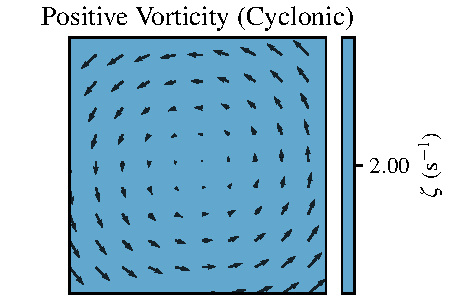
\includegraphics[width=\linewidth]{papers/rossby/images/vorticity_plot3.pdf}\\
        {\small \( \vec{u} = (-y,x),\ \zeta = 2\)}
    \end{minipage}
    \begin{minipage}{0.32\linewidth}
        \centering
        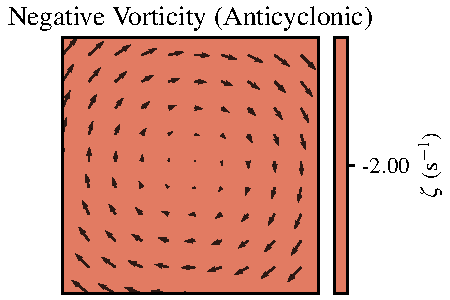
\includegraphics[width=\linewidth]{papers/rossby/images/vorticity_plot4.pdf}\\
        {\small \( \vec{u} = (y,-x),\ \zeta = -2\)}
    \end{minipage}

    \caption{Beispiele für verschiedene Vorticity-Fälle in idealisierten Strömungsfeldern.}
    \label{fig:vorticity_examples}
\end{figure}


	\subsection{Absolute Vorticity}

	Die bisher betrachtete relative Vorticity beschreibt die Rotation eines Luftpakets relativ zum Erdboden.
	Da sich jedoch auch die Erde selbst dreht, muss diese planetare Rotation bei der Beschreibung der Gesamtdrehung berücksichtigt werden.
	Daraus ergibt sich der Begriff der \emph{absoluten Vorticity}, welche die Summe aus relativer und planetarer Vorticity darstellt.

	Die planetare Vorticity wird durch den sogenannten \emph{Coriolis-Parameter} \( f = 2 \Omega \sin \varphi \) beschrieben, wobei \( \Omega \) die Erdrotationsrate und \( \varphi \) die geographische Breite ist.
	Dieser Ausdruck ergibt sich aus der Projektion der Erdrotation auf die lokale Vertikale.
	Die absolute Vorticity ergibt sich somit zu:
	\[
		\eta = \zeta + f
	\]
	wobei \( \zeta \) die relative und \( f \) die planetare Vorticity ist.

	% Die absolute Vorticity ist eine Erhaltungsgrösse in der reibungsfreien, barotropen Atmosphäre, wenn keine vertikalen Bewegungen stattfinden.
	% Sie spielt daher eine zentrale Rolle in der dynamischen Meteorologie und bildet die Grundlage für das Konzept der \emph{potenziellen Vorticity}, welches zusätzlich die Schichtung der Atmosphäre berücksichtigt.

\subsection{Potenzielle Vorticity und ihre Erhaltung}

Die \emph{potenzielle Vorticity} (PV) erweitert das Konzept der \emph{absoluten Vorticity} um die vertikale Struktur der Atmosphäre. 
In ihrer Erhaltungsform ist sie ein zentrales Werkzeug zur Beschreibung grossskaliger Strömungen und Wellenprozesse.

Unter vereinfachten Bedingungen, barotrope, reibungsfreie Atmosphäre mit konstantem Luftvolumen, lautet die Definition:
\[
    q = \frac{\zeta + f}{H},
\]
wobei \(\zeta\) die relative Vorticity, \(f\) den Coriolis-Parameter und \(H\) die effektive Schichthöhe der betrachteten Luftsäule bezeichnet. 
Dieser Ausdruck berücksichtigt sowohl die horizontale Rotation als auch die vertikale Ausdehnung eines Luftpakets.

Ein zentrales Ergebnis der quasi-geostrophischen Theorie ist die Erhaltung der potenziellen Vorticity entlang der Trajektorie eines Luftpakets:
\[
    \frac{Dq}{Dt} = 0.
\]
Unter den genannten Bedingungen treten weder Reibung noch diabatische Wärmeflüsse auf, und die Masse der Luftsäule bleibt erhalten. 
Damit heben sich Änderungen in \(\zeta\), \(f\) und \(H\) entlang der Bewegung eines Luftpakets gegenseitig so auf, dass das Verhältnis \((\zeta + f)/H\) konstant bleibt.

Die PV-Erhaltung erklärt viele grossskalige atmosphärische Phänomene:
Wird ein Luftpaket nach Norden transportiert (höheres \(f\)), so muss es zyklonale Vorticity (\(\zeta > 0\)) abbauen oder sich ausdehnen (\(H \uparrow\)), um \(q\) konstant zu halten. 
Bei einer südlichen Verlagerung gilt der umgekehrte Mechanismus. 
Diese Dynamik ist eine der physikalischen Grundlagen für das Entstehen und die Ausbreitung von Rossby-Wellen, die im folgenden Kapitel behandelt werden.
